
\subsection{Optimized Multicast Implementation}
\label{subsec:merge}

% REVISED STRUCTURE: (a) merger is optimization to \base.  given a set of directed trees, \merge produces small set of fwd rules.  apply to PTs and backup trees, to get less control 
% 		state and faster install.  (b) basic inefficiency, the example,  (c) outline of section
As an optimization to the \base multicast implementation, described in Section \ref{subsec:openflow}, we present the \merge algorithm.  
Given a set of directed trees, produces a near-minimum set of OpenFlow forwarding rules by
consolidating flow table entries at each node where multiple trees use the same set of out-links.  \merge reduces the control state (i.e., number of forwarding rules) necessary to 
multicast packets and, when applied to installing backup trees, can yield faster recovery since fewer control messages are needed to activate backup trees.



%\merge can significantly reduce the control state associated with a multicast tree. At noted in Section \ref{subsec:openflow}, space efficiency is important because OpenFlow switches 
%can only support a limited number of flow table entries.
%Additionally, \merge can yield faster recovery when backup trees are installed using \posts.  Fewer backup tree flow table entries translates to fewer control messages to activate backup trees.

In the next section (\ref{subsubsec:merge-motivate}), we motivate the need for \merge by showing some of the inefficiencies of \bases.  Next, Section \ref{subsubsec:merge-primary} 
presents a simplified version of  \merge that considers only primary trees.  Then, we extend
\merge in Section \ref{subsubsec:merge-backup} to account for backup trees.  Section \ref{subsubsec:merge-discuss} concludes the section with a discussion of how \merge affects garbage
collection and \pcnts, along with informal commentary on its optimality.
%optimality, and complexity.

\begin{figure}
  \centering
   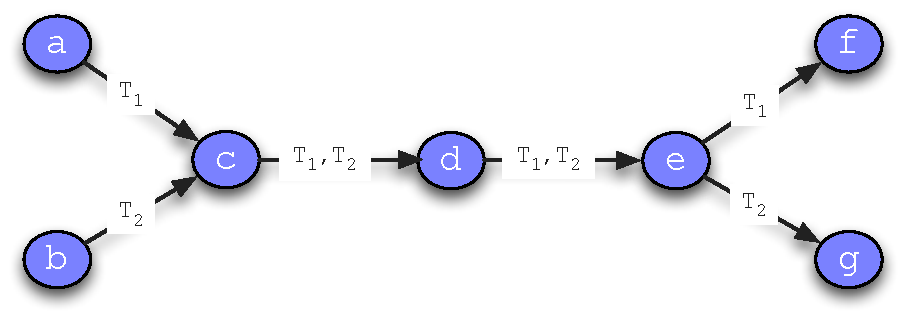
\includegraphics[scale=0.55]{figs/merger-example.pdf}
\caption{Example showing a subtree of two multicast trees, $T_1$ and $T_2$.  The edges used by each multicast tree are marked.}
\label{fig:merger-example}
\end{figure}


\subsubsection{Motivation: \basen Algorithm Inefficiencies}
\label{subsubsec:merge-motivate}

The \base multicast implementation creates a flow table entry at each node of a multicast tree that matches using the tree's multicast address. 
As a result, a switch, $v$, may have multiple flow table entries executing the same actions.  This occurs when multicast trees share the same outgoing links at $v$. 
\footnote{In cases where the tree can either be a primary tree or backup tree, we refer to the tree as a multicast tree.}
These inefficiencies are the motivation for developing the \merge algorithm, which replaces the set of flow table entries \base would create at $v$ with a single flow table entry. 
To do so, \merge writes a common identifier, or tag, in packet headers at the node immediately upstream from $v$. Using this tag, \merge creates a \emph{single} rule at $v$ to match and 
forward packets of \emph{all} trees with the same outgoing links at $v$.

Consider the simple example shown in Figure \ref{fig:merger-example} with two multicast trees $T_1$ and $T_2$. The directed links used by each tree are marked.
\base creates a flow table entry for $T_1$ at $a$, $c$, $d$, $e$, and $f$ and a flow table entry at $b$, $c$, $d$, $e$, and $g$ for $T_2$.  Because 
$T_1$ and $T_2$ both use the same outgoing links at $c$ and $d$, only a single forwarding rule is needed at each node.  This is what \merge creates and in the next two sections we describe how.

%In contrast, \merge leverages that $T_1$ and $T_2$ both use the same outgoing links at $c$ and $d$ to replace the two separate flow table entries at $c$ and $d$, created under \bases, with a single 
%forwarding rule. To do so, \merge first creates an action at $a$ and $b$ to write an identifier in the packet headers of all packets traversing $(a,c)$ and $(b,c)$.
%Then, at $c$ and $d$, \merge creates a single rule to match and forward packets based solely on this tag.




\subsubsection{\mergen Algorithm for Primary Trees}
\label{subsubsec:merge-primary}


\merge consolidates flow table entries at each node, $v$, where multiple primary trees share the same outgoing links. 
Upstream from $v$, \merge writes an identifier, or \emph{tag}, in packet headers and uses this tag to match packets at $v$ using a single rule shared by each of these primary trees.
%An identifier, or \emph{tag}, is used to match packets at $v$.  
%\merge writes this tag in the packet header at the node immediately upstream from $v$. % in the packet header of all packets corresponding to any of these multicast trees. 
The tag is removed downstream from $v$ where the trees diverge. 

A tag is a globally unique Ethernet address \merge writes in a packet header's {\tt dl\_dst} field (i.e., the Ethernet destination address).  When possible, \merge flow table entries use 
tags to match and forward packets, meaning that packets are matched solely on their {\tt dl\_dst} value.
When the same Ethernet address is applied to the packets of more than one multicast tree, we refer to this as a \emph{group tag}.  A \emph{single tag} is an 
Ethernet address used by only one tree. We use the term \emph{tag} to generically refer to either a group or single tag.
%\footnote{In some cases, packets corresponding to a multicast tree $T_i$ already have a tag written in their packet header upon reaching node $u$.  If this same tag is used to match packets 
%at $d$ where $(u,d) \in T_i$ no action is created at $u$ to write this same tag. However, for ease of explanation, we say that \merge writes the tag at $u$.}

\begin{figure}
  \centering
   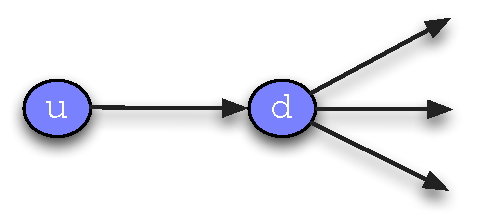
\includegraphics[scale=0.5]{figs/merger-ud.pdf}
\caption{Subgraph used to describe \merge in Section \ref{subsubsec:merge-primary}.}
\label{fig:merger-ud}
\end{figure}

%With these preliminaries in place, 
We are now ready to describe \merge in more detail.  
First, \merge marks the edges used by each primary tree.  Then, \merge executes a breadth first search of each primary tree, $T_i$, starting at its root.  
For each link $(u,d) \in T_i$ as shown in Figure \ref{fig:merger-ud}, \merge determines the match pattern to create at $d$ and the tagging actions to apply at $u$ using the following steps:
\footnote{Because $T_i$ is a tree, $(u,d)$ must be its only incoming link to $d$.  Therefore, we can determine $T_i$'s locally optimal tagging rule at $d$ by only considering $u$ and $d$.}
\begin{enumerate}

	\item Finds the set of trees, $S$, using $(u,d)$ that share the same outgoing links as $T_i$ at $d$. 

	\item If $|S| \geq 1$, \merge creates an action to write a group tag at $u$.  For each $T_j \in S \cup \{T_i\}$, \merge finds the rule at $u$ used to forward $T_j$ and appends an action
	to write a group tag to the rule's action list.
	Then, a single rule is created at $d$ that matches packets using this group tag and has an initial action list forwarding packets out the appropriate ports.

	\item If $S = \emptyset$, \merge peaks upstream at $u$ to determine whether to use a single tag or $T_i$'s multicast destination address to match $T_i$'s packets at $d$. 
	When $T_i$ is matched using either a single tag or its multicast destination address at $u$, \merge creates a rule at $d$ to match packets using a single tag and writes this single
	tag at $u$.  Otherwise, \merge creates a rule at $d$ matching packets using $T_i$'s multicast destination address (no action is needed at $u$).  
	%\footnote{If we were to write $T_i$'s single tag at $u$, this tag would be erroneously be applied to any other multicast tree using the same group tag as $T_i$ to match packets at $u$. }
	%Only when $T_i$ is matched using either a single tag or its multicast destination address at $u$, do we create a rule at $d$ to match packets using $T_i$'s single tag.  In which case, 
	%an action is created at $u$ to write this single tag.

\end{enumerate}
In step (3), we aim to use single tags to match packets because they allow \emph{any} backup tree to reuse $T_i$'s rule at $d$ by simply writing this tag at $u$.  
Whereas, if $T_i$'s multicast address is used to match packets at $d$, only $T_i$'s backup trees can reuse this forwarding rule (since $T_i$'s multicast address is unique to its multicast group).
We comment further on this design decision in the next section.

%In the Figure \ref{fig:merger-example} example, \merge leverages that $T_1$ and $T_2$ both use the same outgoing links at $c$ and $d$ to create a single rule at each node (as opposed
%to two separate flow table entries that would be created with \bases).  %After marking the edges used by $T_1$ and $T_2$, \merge
In the Figure \ref{fig:merger-example} example, \merge  creates an action at $a$ and $b$ to write a group tag in the packet headers of all packets traversing $(a,c)$ and $(b,c)$.
Then, at $c$ and $d$, \merge creates a single rule to match and forward packets based solely on this tag.  With regard to the breadth-first search (BFS) described earlier, 
\merge executes the following steps in  its breadth-first search (BFS) of $T_1$ at nodes $c$, $d$, and $e$.
%We describe the steps \merge executes in its breadth-first search (BFS) of $T_1$ at nodes $c$, $d$, and $e$.
At $c$, $S=\{T_2\}$ so \merge finds $T_1$'s rule at $a$ and includes an action to write a group tag, {\tt 12}, in all packets sent out $a$'s port to $c$. 
Then, \merge creates a flow table entry at $c$ that matches packets with {\tt dl\_dst = 12} and forwards packets out the port to $d$.  The same set of actions occur when the BFS reaches $d$. 
%except that no group tag needs to be written at $c$ because the same group tag
%At $e$, $S=\emptyset$ because $T_1$ and $T_2$ diverge. at $e$.  
\merge creates a forwarding rule at $e$ that matches packets using $T_1$'s multicast address and forwards these packets to $f$.



\subsubsection{\mergen Algorithm for Backup Trees}
\label{subsubsec:merge-backup}

Having discussed \merge for the primary tree case, we are now ready to extend \merge to generate forwarding rules for backup trees.  \merge 
aims to reuse forwarding rules of primary trees because these rules are already installed in the network, allowing the installation algorithm
(e.g., \pre or \posts) to avoid installation a new forwarding rule.  In cases where primary tree rules cannot be reused, \merge consolidates
flow table entries with other backup trees that have common forwarding behavior.

%We describe the case of generating forwarding rules for a set of backup trees, $\hat{T}^l$, using $l$. 
For a set of backup trees, $\hat{T}^l$, \merge generates backup tree forwarding rules as follows. 
\merge executes two rounds of BFS, traversing all
$\hat{T}^l_i \in \hat{T}^l$ in each round.  In the first round, for each $\hat{T}_i^l$, \merge finds each node where $\hat{T}_i^l$ has the same outgoing links as a primary tree.  
If so, $\hat{T}_i^l$ reuses the primary tree flow table entry at this node, $v$: \merge writes the primary tree tag at $v$'s parent node
allowing $\hat{T}_i^l$ packets to be forwarded using the primary tree rule, and makes no changes at $v$.

In the second round of BFSs, \merge consolidates flow table entries among the other backup trees for $l$
at nodes where primary tree tag reuse was not possible.  
To do so, the algorithm from Section \ref{subsubsec:merge-primary} is executed but comparing $\hat{T}_i^l$'s outgoing links with the outgoing links of 
each $\hat{T}_j^l \neq \hat{T}_i^l$ at nodes where $\hat{T}_i^l$ and $\hat{T}_j^l$ were unable to reuse primary tree tags. 

When \merge is applied to \pre and \post (referred to as \pres+\merge and \posts+\merges) the tag becomes the sole match criteria used by its flow table entry, with one exception.  This 
occurs with \pres+\merge when a {\tt bid} is required to distinguish between a backup and primary tree, as described in Section \ref{subsec:install-backups}. In those cases, the 
{\tt bid} and {\tt dl\_dst} fields are both used as match criteria.

%\merge attempts to reuse flow table entries of primary trees already installed in the network that share forwarding behavior with a backup tree. 
%First, \merge attempts to reuse flow table entries of primary trees already installed in the network that share forwarding behavior with a backup tree.  At nodes where this possible, no 
%flow table entry needs to be installed.  At the remaining nodes, % At nodes where this is not possible,
%\merge applies the procedure from Section \ref{subsubsec:merge-primary} to consolidate forwarding rules with other backup trees.  We detail these steps below. % for backup trees of link $l$.



%Under \merge we can avoid matching using a tree-id at any $d \in D^l_i$ where $\hat{T}_i^l$ uses a group tag or reuses a primary tree tag. 
%These tags are applied upstream from $d$ and are different from any tags $T_i^l$ uses  a $d$.  The tree-id is only required at $d \in D^l_i$ where \merge is forced to 
%match $\hat{T}_i^l$'s multicast address or single tag.  \merge described in Section \ref{subsec:merge-backup}, is modified to incorporate this additional match criteria. 

\subsubsection{\mergen Discussion}
\label{subsubsec:merge-discuss}

%Now that we have presented the core of aspects of \merges, we comment on. We comment on a number of 
To unify our presentation of \merges, we comment on some of the properties of the algorithm along with the implications of using \merge on other important aspects of \mdrs.
%In the following order, we discuss the advantages of using \merges, \merge time complexity, \merges's implications on garbage collection, \merges's ``do not harm'' property, and
%how \pcnt monitors \merge flows. 

{\bf Benefits.}
In comparison with \bases, \merge reduces the number of forwarding rules required to install each multicast tree.  As a result,
\merge is more space efficient and can yield faster backup tree installation.
%By reducing the number of forwarding rules required to install each multicast tree, \merge is more space efficient and can yield faster backup tree installationi with \posts+\merges.
Recall that for each primary tree, \mdr pre-computes a backup tree for each of its links.  In this scenario \pres+\merge can significantly reduce the number of pre-installed rules.
These savings are especially important because, as noted in Section \ref{subsec:openflow}, OpenFlow switches can only support a limited number of flow table entries.
With \posts, \merge can yield faster recovery because fewer backup tree flow table entries translates into fewer control messages to activate backup trees.

{\bf Time Complexity.}
Like \bases, \merge complexity is bounded by the breadth-first search (BFS) executed for each of the $m$ multicast trees given as input.  At each node, $v$, visited in the BFS, \merge
compares the out-links used by all other multicast trees that use $v$.  Since there can be at most $m$ such trees, this takes $O(m)$ time.  If we let $n$ be the number of graph nodes,
each BFS takes $O(mn)$ time \footnote{BFS has $O(|V|+|E|)$ complexity. In our case, each BFS is over a directed tree, meaning the number of edges traversed in each BFS is $O(n-1)$.  
Therefore, we can simplify BFS time complexity to $O(n)$.}
and the total time complexity of \merge is $O(m^2n)$.

% O( V+E), is O(V) because we are dealing with trees
% each BFS step has O(m) complexity, since need to check the out-links of all other trees using v
%  m x O(mn) -- O(m^2n)

{\bf Garbage Collection}.
\mdrs's garbage collection algorithm remains unchanged from the description in Section \ref{subsec:garbage}.  
Recall that {\tt rule\_map} is a dictionary that maps the flow table entry installed at each node to the
set of backup and primary trees using the flow table entry. The only difference between \base and \merge garbage collection is the number of stale rules it identifies (likely fewer
stale rules with \merges) not how the stale rules are found.  
As with \bases, \merge garbage collection can find any stale forwarding rules by consulting {\tt rule\_map}.


%Garbage collection
%Under our \base multicast implementation, garbage collection is straightforward.  The controller maintains a dictionary, {\tt rule\_map}, for each node, mapping
%each multicast tree (primary tree and backup trees) using $v$ to the flow table entry installed at $v$. When a link, $l$, fails the garbage collection routine determines 
%the set of stale forwarding rules for each $T^l_i$. A stale rule exists at each $v \in V_i \setminus \hat{V}_i^l$ (i.e., nodes unique to the primary tree) and each $d \in D_i^l$ 
%(nodes where the backup tree diverges from the primary tree).  The controller consults {\tt rule\_map} to find the forwarding rule at each node and either sends an explicit 
%remove flow message to each of these nodes (if using a hard state signaling scheme \cite{HardSoftState}) or allows the forwarding rule to time out (with a soft state algorithm \cite{HardSoftState}).

%With \merges, garbage collection adds an additional check before removing any candidate stale flow table entry, $c_v$, found using the procedure described in the previous paragraph.  
%Garbage collection consults {\tt rule\_map} to determine if any other primary tree or newly installed backup tree uses $c_v$, if so 
%is modified to check that no other primary tree 

%\merge complicates garbage collection because it is no longer the case that an installed flow table entry is used by a single multicast tree (e.g., multiple primary trees
%can share the same flow table entry).  Garbage collection must now consider that a different set of primary trees
%use flow table entry, $e$, before $l$ fails versus after $l$ fails and backup trees $\hat{T}^l$ are installed.  To account for this, we modify the first step of garbage collection.  
%Rather than simply add $T_i$'s flow table entry, $e_v$, at each $v$ to $E_r$, the garbage collection first checks if any newly installed tree (i.e., each tree in $\hat{T}^l$) reuses $e_v$. Then, we
%check if any primary tree unaffected by $l$ failing (i.e., each tree in $\bar{T}^l$) uses $e_v$. If either of these checks is positive, $e_v$ is 
%not included in $E_r$ but {\tt flow\_map} is updated for $T_i$.  Otherwise, $e_r$ is added to $E_r$ and {\tt flow\_map} is updated for $T_i$.

%\item \underline{Garbage Collection}: keep track of flows used by each tree.  garbage collection ensures flows of unaffected trees are not removed.

{\bf Do No Harm.} 
We say that \merge is an algorithm that does ``no harm''  \footnote{This is similar in spirit to the Hippocratic Oath taken by physicians that they will ``never do harm [to patients]'' }
because (a) \merge never creates more flow table entries than \base and (b) when generating rules for backup trees, \merge makes no modifications to flow table entries of primary trees that do not use the 
failed link. We informally prove each of these properties below.

Regarding (a), consider an arbitrary multicast tree (primary of backup tree), $T_i$. \merge creates at most one flow table entry at any $v \in T_i$.  
The flow table entry, $e_i$, either matches and forwards packets using a group tag, a single tag, or using the $T_i$'s multicast address.  Any $e_i$ tagging actions 
are simply appended to $e_i$'s action list (when \merge visits $T_i$'s children of $v$), requiring the creation of no additional flow table entries.  We conclude that in the worst case,
\merge creates the same number of flow table entries as \bases.  

Now consider property (b) where we let $T_j$ refer to a primary tree not using $l$. By construction, \merge only creates flow table entries and new actions for the backup trees of 
link $l$ (i.e., $\hat{T}^l$). These flow table entries have distinct match criteria than those \merge creates for $T_j$.  If a backup tree reuses $T_j$'s flow table entry at $v$, 
no changes are made to this flow table entry.  Lastly, \mdrs's garbage collection algorithm ensures that no $T_j$ flow table entry is removed.

%As an aside, \merges's do no harm property ensures that under \merges, garbage collection has fewer flow table entries to remove than with \bases.  Intuitively, this 
%is reasonable because \merge seeks to reuse primary tree flow table entries. 


{\bf Optimality}.  
Because \merge makes tagging decisions locally at each node, $v$, based only on the multicast trees using $v$'s outgoing links and the tags used at $v$'s parent nodes,
\merge does not always yield the minimum set of forwarding rules.
Consider again Figure \ref{fig:merger-example} but replace $T_1$ with $S_1$ and $T_2$ with $S_2$, where $S_1$ and $S_2$ are sets of multicast trees of size $k$.
%$S_1=\{T_1,T_2,...,T_k\}$ and $S_2 = \{T_{k+1},T_{k+2},...,T_{2k+1}\}$.  
In this scenario, \merge writes the same group tag, denoted {\tt 12}, at $a$ and $b$ for each tree in $S_1$ and $S_2$.  Then, at $c$ and $d$ \merge installs a single rule that matches and forwards 
using the {\tt 12} tag.  Lastly, for each $T_i \in S_1 \cup S_2$, a rule is created at $e$ that matches packets using each $T_i$'s multicast address.  %This results in 

A better solution in this example is to use a different group tag for $S_1$ and $S_2$.  Under this proposal, let {\tt 11} be the group tag applied to each tree in $S_1$ 
at $a$ and {\tt 22} the tag we write 
in the packet header of each tree in $S_2$.  These group tags can be used create two separate rules at $c$, $d$, and $e$ to forward $S_1$ packets based on {\tt 11} and $S_2$ packets using {\tt 22}.
By using different tags for $S_1$ and $S_2$, we avoid having to create $2k$ separate rules for each tree in $S_1 \cup S_2$ at $e$, clearly a better solution that the 
one produced by \merges. 

This example suggests that an algorithm, $\mathcal{A}$, that finds the minimum number of forwarding rules for a set of multicast trees $T$ 
must consider, for $S \subseteq T$ where each multicast tree $S_i \in S$ uses link $(u,d)$, how each of $S$'s subsets share links downstream from $d$.
Since this requires computing the power set of $S$ and there are an exponential number of ways $S$'s subsets can use common links downstream from $d$,
we conjecture that no polynomial time $\mathcal{A}$ exists. %a polynomial time algorithm that yields the optimal  solution does not exist.





%The single group tag used at u forces a separate rule to be created for each tree in S if not all S have the same outports at d.  In some cases, it is beneficial to partition S into subsets, 
%based on links shared downstream, and use a group tag unique to each subset to match and forward packets downstream. 

%Consider the following example.  S_1 and S_2 denote a set of trees and let S = S_1 \cup S_2.   Merger creates an action at a and b to write group tag, denoted 12,  for each tree in S_1 and S_2.  Then, at u a single rule matches and forwards using the 12 tag.  Lastly, a rule is created at d for each tree in S that matches using the tree's destination address to ensure correct forwarding at d.  A better approach is to write group tag 11 at a for S_1 and group tag 22 for S_2 at b.   We can use these group tags to match and forward -- using two separate rules -- at u and d using group tags 11 and 22.   Using different tags for S_1 and S_2 makes it unnecessary to create a separate rule for each tree in S at d.   The same challenge arises if u and d were connected using additional links all used by S. 

{\bf Implications for \pcnts.}
\pcnt requires no changes to monitor packet loss of flows forwarded using \merge rules. However, we make 
the case here that \merge can improve the accuracy of \pcnt loss rate estimates and reduce the time to compute these estimates.  In Section
\ref{subsec:eval-pcount}, we will find that our simulations bear out the qualitative argument made here.

% (a) can tune k.  cost associated with each k
Recall from Section \ref{subsec:pcnt} that with \pcnt the number of monitored flows, $k$, can be tuned.
Determining an appropriate $k$ parameter involves a trade-off between the accuracy of packet loss estimates and time: larger $k$ yield more accurate packet loss estimates
but at the cost of slower detection times (the time between when packet loss occurs and when it is detected). Detection times of a monitored link, $(u,d)$, increase with larger $k$
for two reasons. One, for each of the $k$ flows, \pcnt makes a copy of the flow's forwarding rule at $u$ and $d$ in order tag and count packets.  Two, 
\pcnt sends $k$ queries to $u$ to read the state of each flow table entry generated by \pcnts. % generated flow table entry and a single aggregate statistic query to $d$.

%a function of the number of statistic queries \pcnt sends. % to the switches of a monitored link.  
%Recall from Section \ref{subsec:pcnt}, when estimating packet loss of a link, $(u,d)$, \pcnt makes a copy of the flow table entry at $u$ and $d$, for each flow \pcnt monitors. 

With \merge the same flow table entry, $e_i$, can be used by multiple ($r$) flows.  In these cases, \pcnt only needs to explicitly monitor one of these flows to measure
the packet loss of all $r$ flows.  That is, \pcnt can monitor the loss of all $r$ flows with cost of monitoring a single flow:
the one copy of $e_i$ \pcnt makes at $u$ and $d$ ensures that packets of any of these $r$ flows are tagged and counted and
only a single statistic query is needed to retrieve $e_i$'s packet count.

Consider the example in Figure \ref{fig:intuition-example-t1} and suppose that \pcnt monitors link $(g,l)$. 
Two multicast flows -- $f_b$ for primary tree $T_b$ and $f_c$ for primary tree $T_c$ -- traverse
$(g,l)$.  \base creates a separate forwarding rule for $f_b$ and $f_c$ at $g$ while \merge generates a single forwarding rule at $g$ used by both $f_b$ and $f_c$.  As a result, 
with \merges, \pcnt can track the  packet loss of $f_b$ and $f_c$ by querying just the shared \merge forwarding rule at $g$ (rather than interact with two separate \base forwarding rules).
These savings are quantified using simulations in Section \ref{subsec:eval-pcount}.

%Recall from Section \ref{subsec:pcnt} that with \pcnt the number of monitored flows, $k$, can be tuned.  Determining an appropriate $k$ parameter involves a trade-off between the accuracy of
%packet loss estimates and time: larger $k$ yield more accurate packet loss estimates but at the cost of slower detection times (the time between when packet loss occurs and when it is detected).
%Detection times of a monitored link, $(u,d)$, are a function of the number of statistic queries \pcnt sends. % to the switches of a monitored link.  
%\pcnt sends a read state query for each monitored flow to $d$ and a single statistic query to $d$.

%As a mechanism to count packet loss, \pcnt makes a copy of the flow table entry of each monitored flow where the flow table entry copy upstream tags packets upstream and a second flow table entry copy counts 
%tagged packets downstream.  Because with \merge the same flow table entry, $e_i$, may be shared by multiple flows, all of these flows can be monitored at the cost of monitoring a single flow: 
%only a single \pcnt statistic query is needed to retrieve $e_i$'s packet count rather than one separate query per flow using $e_i$ that would necessary with \bases.  



